% Author: Dr. Matthias Jung, DL9MJ
% Year: 2020
\documentclass[convert = false, border=5pt]{standalone}
\usepackage{fontspec}
\setmainfont{Roboto}
\usepackage[siunitx, straightvoltages]{circuitikzgit}
\usepackage{tikz}


\usepackage{tikz,pgfplots}
\usepgfplotslibrary{fillbetween}

\begin{document} 
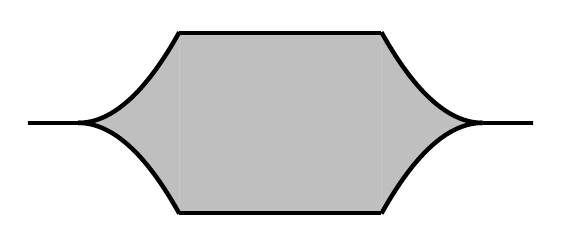
\begin{tikzpicture}
    \pgfplotsset{samples=200}
    \begin{axis}[
        width=8cm,
        height=4cm,
        axis lines=none,
        ticks=none,
        xmin =  0,
        ymin = -1.4,
        xmax =  10,
        ymax =  1.4,
        domain = 0:10,
        thick,
        smooth,
        no markers]
        \addplot+[solid, name path=X,ultra thick, black, domain=0:1]
        { 0};
        \addplot+[name path=A,ultra thick, black, domain=1:3]
        { 1/3*(x-1)^2};
        \addplot+[name path=B,ultra thick, black, domain=1:3]
        {-1/3*(x-1)^2};
        \addplot[gray, opacity=0.5, domain=1:4] fill between[of=A and B];
        \addplot+[name path=C,ultra thick, black, domain=3:7]
        { 1.325};
        \addplot+[solid, name path=D,ultra thick, black, domain=3:7]
        {-1.325};
        \addplot[gray, opacity=0.5, domain=3:4] fill between[of=C and D];
        \addplot+[solid, name path=E,ultra thick, black, domain=7:9]
        { 1/3*(x-9)^2};
        \addplot+[solid,name path=F,ultra thick, black, domain=7:9]
        {-1/3*(x-9)^2};
        \addplot[gray, opacity=0.5, domain=6:8] fill between[of=E and F];
        \addplot+[name path=X,ultra thick, black, domain=9:10]
        { 0};
    \end{axis}
\end{tikzpicture}
\end{document}

